
\section{\ref{PS:Q:Availability}}
\subsection{Experiment}
The \ref{PS:Q:Availability} question asks if the proposed decentralized system is able to continue its functions even though nodes are removed from the system at runtime.
The proposed decentralized system should be able to continue maintaining the global setpoint of the park even if some turbines become unavailable, this of course assumes that available capacity is present in the park.

The below experiment is repeated with a N failing turbines
The experiment has the following procedure:
$N = 1, 5, 10, 15$
\begin{enumerate}
	\item Start the system with 30 turbines.
	\item Make sure the system is stable.
	\item Kill N nodes.
	\begin{itemize}
		\item did the system discover the failed node within a 150ms timeframe?
		\item did the system adjust the setpoints for all turbines to maintain the global setpoint?
	\end{itemize}
\end{enumerate}

\subsection{Results}
\label{sec:res:availability}
The plots in \cref{fig:exp:availability_kill15,fig:exp:availability_kill10,fig:exp:availability_kill5,fig:exp:availability_kill1} show how the decentralized solution reacts when killing 1, 5, 10 and 15 turbines. To begin with there are 30 turbines, the setpoint is set to 2,000 for all setups except for when killing only one turbine(\cref{fig:exp:availability_kill1}) it was set to 20,000. This was done so that it was possible to visually verify that the turbines reacted.
The turbines are all running with a cycle time of 20 ms.

\begin{figure}
	\centering
	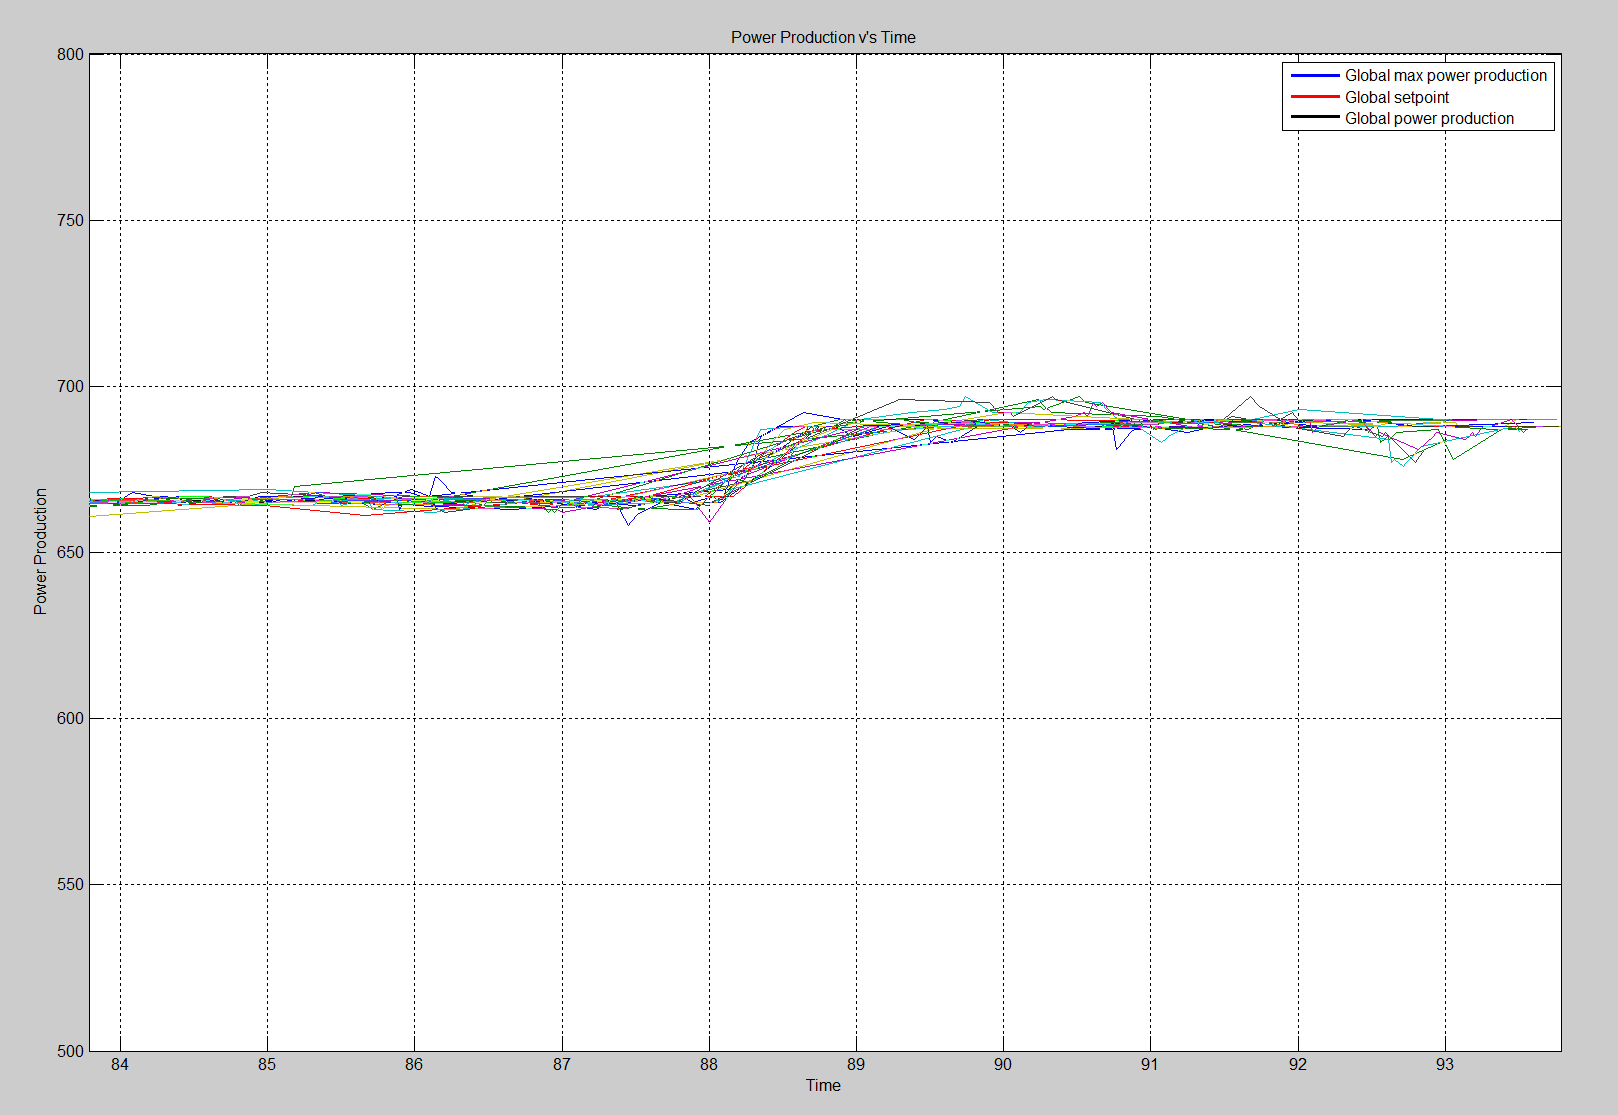
\includegraphics[width=\resultsFigureWidthScale\textwidth]{figures/Results/availabilitytest30-29_setpoint_20000.PNG}
	\caption{Availability test kill 1 out of 30 turbines}
	\label{fig:exp:availability_kill1}
\end{figure}

\begin{figure}
	\centering
	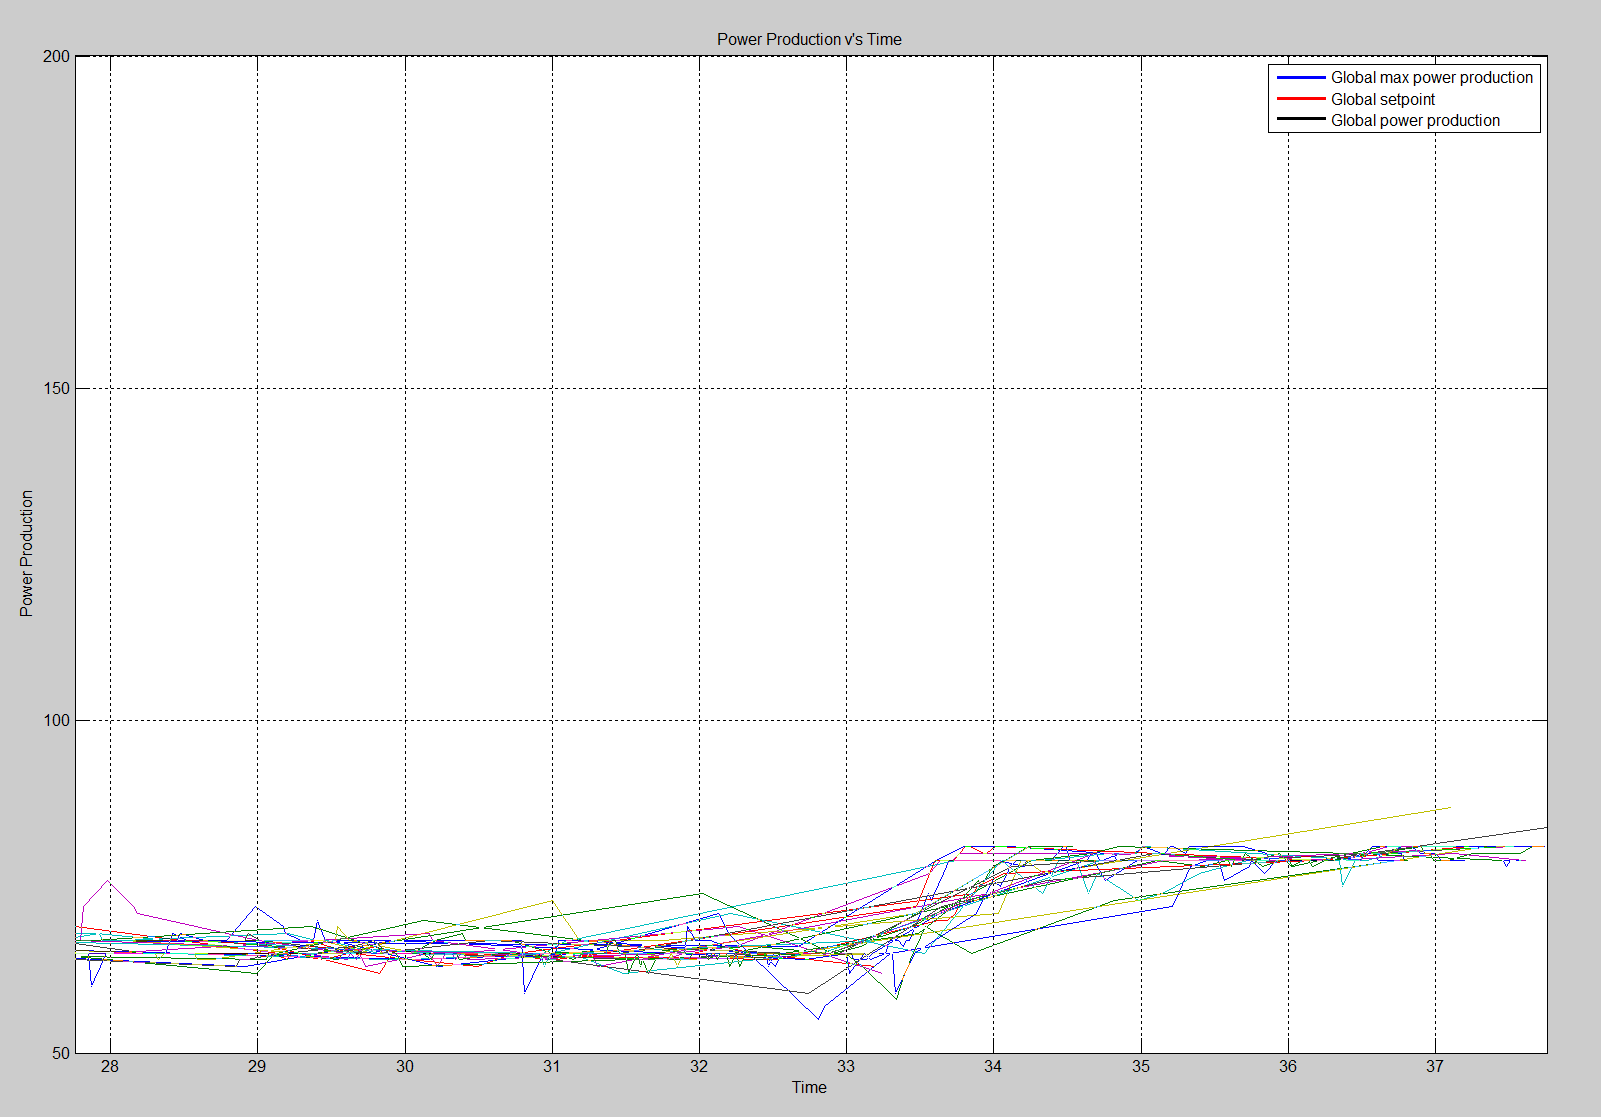
\includegraphics[width=\resultsFigureWidthScale\textwidth]{figures/Results/availabilitytest30-25_setpoint_2000.PNG}
	\caption{Availability test kill 5 out of 30 turbines}
	\label{fig:exp:availability_kill5}
\end{figure}

\begin{figure}
	\centering
	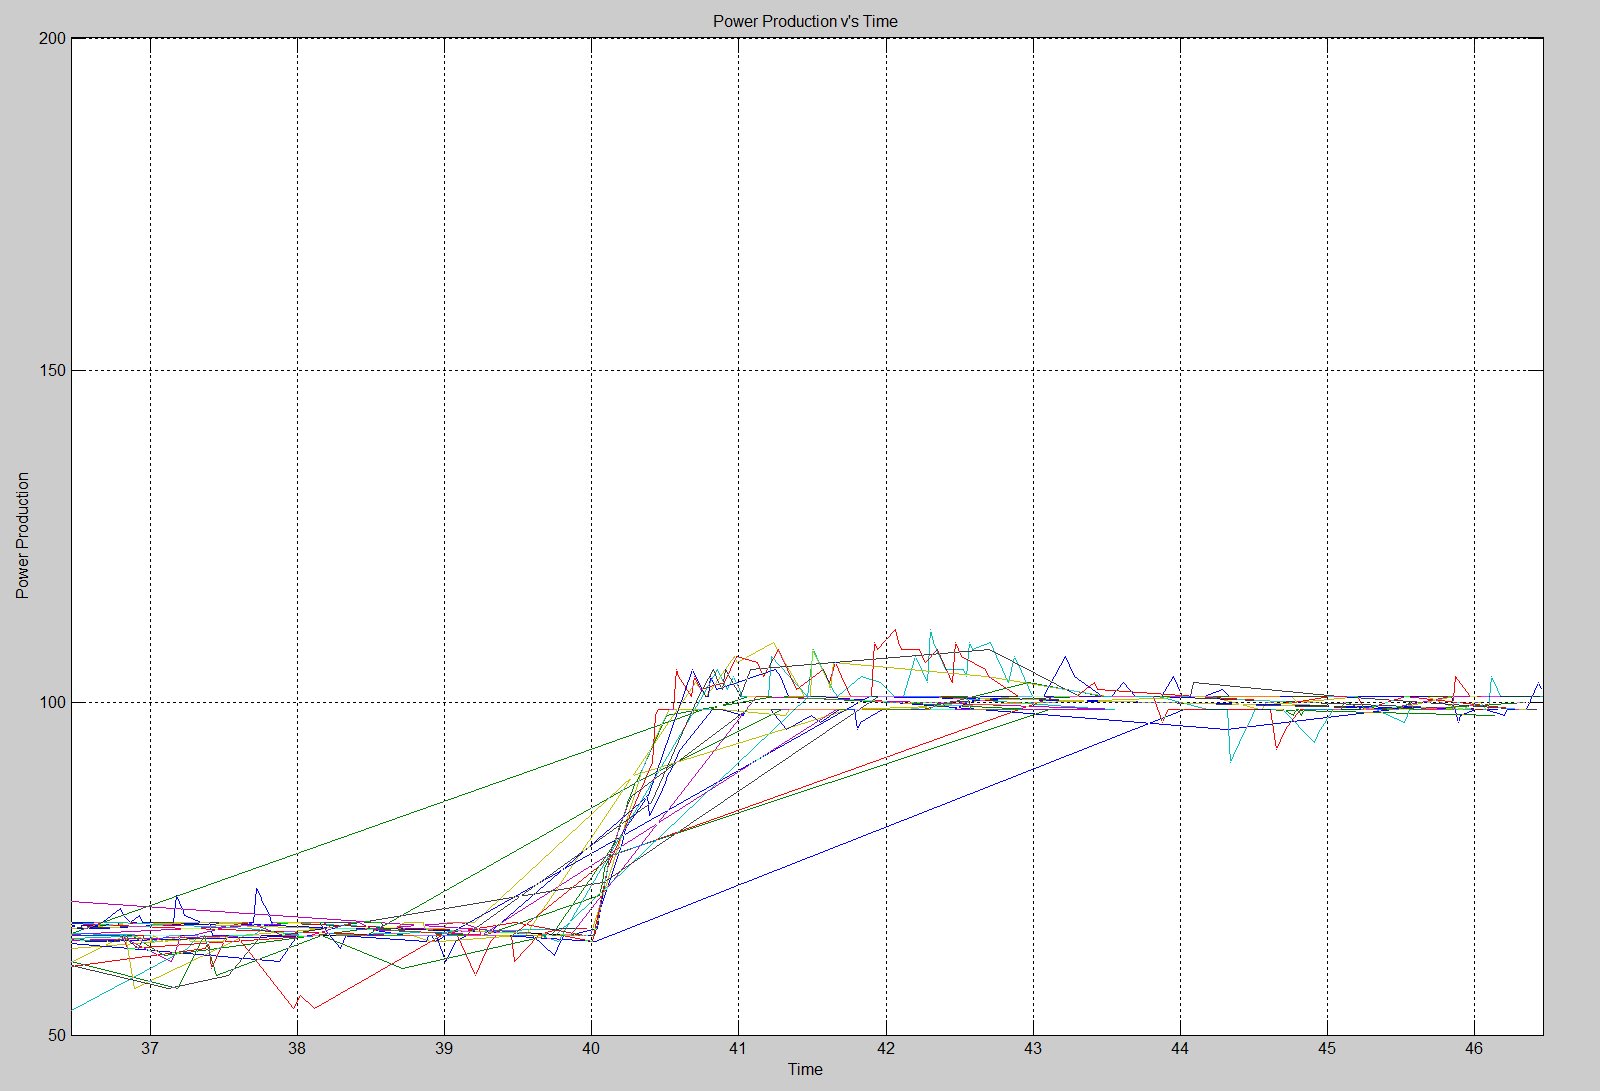
\includegraphics[width=\resultsFigureWidthScale\textwidth]{figures/Results/availabilitytest30-20_setpoint_2000.PNG}
	\caption{Availability test kill 10 out of 30 turbines}
	\label{fig:exp:availability_kill10}
\end{figure}

\begin{figure}
	\centering
	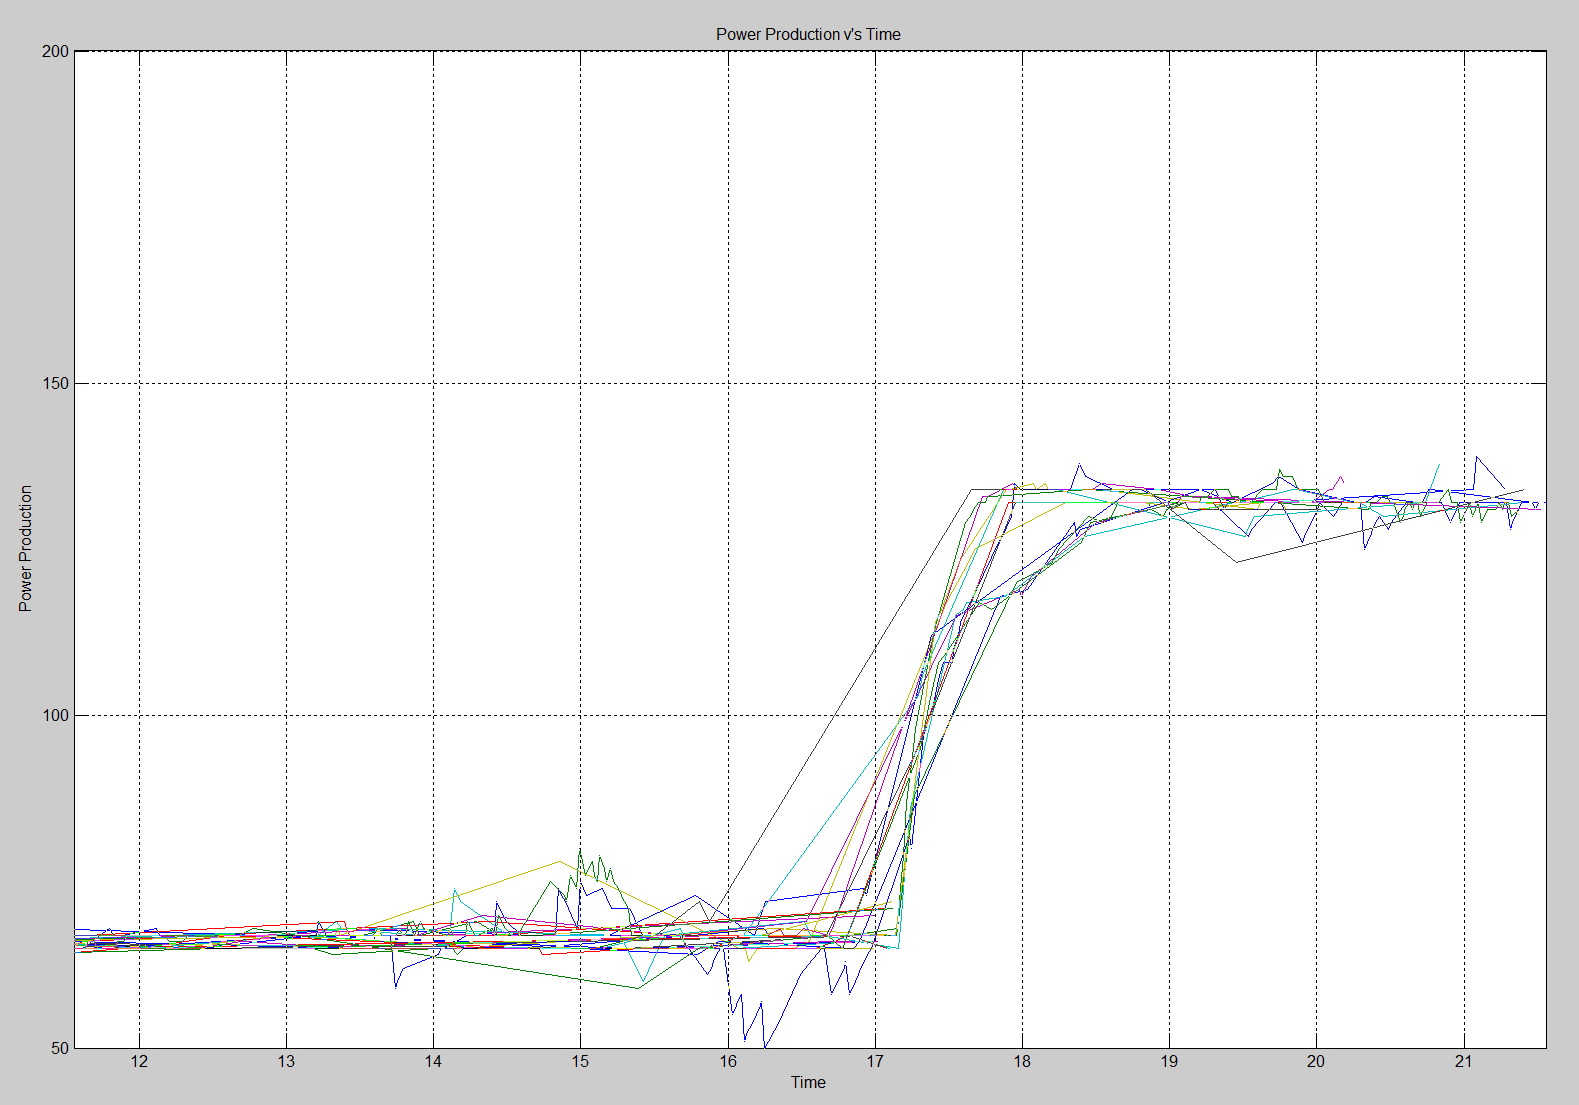
\includegraphics[width=\resultsFigureWidthScale\textwidth]{figures/Results/availabilitytest30-15_setpoint_2000.PNG}
	\caption{Availability test kill 15 out of 30 turbines}
	\label{fig:exp:availability_kill15}
\end{figure}


\subsection{Discussion}

